\documentclass[11pt,a4paper,addpoints]{exam}

% Essential packages
\usepackage{amsmath, amssymb, amsthm}
\usepackage{graphicx,color}
\usepackage[left=1in, right=1in, top=0.8in, bottom=.8in, includefoot, headheight=13.6pt]{geometry}
\usepackage[square, comma, numbers, sort&compress]{natbib}
\usepackage[T1]{fontenc}
\usepackage{caption}

% Optional customization packages
\usepackage{lmodern}

% Tables
\usepackage{xcolor}
\usepackage{colortbl}

\newcommand{\mc}[2]{\multicolumn{#1}{c}{#2}}
\definecolor{Gray}{gray}{0.83}

\newcolumntype{a}{>{\columncolor{Gray}}c}
\newcolumntype{b}{>{\columncolor{white}}c}

\begin{document}
\pagestyle{headandfoot}
\runningheadrule
\firstpageheader{EC-102 -- CSP Lab}{Quiz 0-A}{\today}
\runningheader{EC-102 -- CSP Lab}
{Quiz 0-A, Page \thepage\ of \numpages}
{\today}
\firstpagefooter{}{}{}
\runningfooter{}{}{}

\fbox{\fbox{\parbox{5.5in}{\centering
Read each question carefully and \emph{encircle} the appropriate choice.}}}

\vspace{0.2in}
\makebox[0.44\textwidth]{Name:\enspace\hrulefill}~~~\makebox[0.44\textwidth]{Reg. No.\enspace\hrulefill}\\
\vspace{0.2in}
\makebox[\textwidth]{Instructor:\enspace Usman Ayub Sheikh}

\begin{questions}
    \question [1] The only language that is \emph{completely} understood by computers is \fillin.
        \begin{choices}
            \choice C++
            \choice Assembly language
            \choice english language
            \choice machine language
        \end{choices}

    \question [1] Every C++ program \emph{must} contain one ~\fillin~ function.
        \begin{choices}
            \choice cout
            \choice main
            \choice using
            \choice int
        \end{choices}

    \question [1] Which of the following is \emph{not} a C++ data type?
        \begin{choices}
            \choice int
            \choice single
            \choice float
            \choice char
        \end{choices}

    \question [1] Which of the following is \emph{not} a C++ logical operator.
        \begin{choices}
            \choice $\&\&$
            \choice $!=$
            \choice $||$
            \choice $!$
        \end{choices}

    \question [1] Which of the following expressions has \emph{not} been computed correctly.
    \begin{table}[!htb]
        \centering
        \begin{tabular}{abb}
            \hline
            \rowcolor{Gray}
            & \textbf{Expression} & \textbf{Computes to} \\
            \hline
            A & \texttt{(2.5 < 2.6 \&\& `c' != `C')}  & 1 \\
            B & \texttt{(1 || `d' > `c' \&\& 1)} & 1 \\
            C & \texttt{(1 <= 6 \% 2 \&\& 2.05 > 20.5)} & 0 \\
            D & \texttt{!(`x' <= `y' || `x' >= `y' \&\& 5.5 > 3)} & 0 \\
            E & \texttt{(`c' != `C' \&\& 25 > 24 || `a' > `b')} & 0 \\ \hline
        \end{tabular}
    \end{table}

    \question [5] Obesity can cause a number of problems including diabetes and heart disease. In order to determine whether a person is overweight or obese, a measure known as Body Mass Index (BMI) is used. BMI is defined as: \\
    \begin{equation*}
        BMI = \frac{weight}{height^2}
    \end{equation*}
    where weight is taken in kilograms and height in meters.

    \par
    In this problem, you are required to answer a few questions related to a program that takes \textit{height} and \textit{weight} of the user as an input, calculates his/her BMI, and displays a message such as ``underweight'', ``healthy'', ``overweight'' or ``obese'' based on the following graduation:
        \begin{table}[!htb]
        \centering
        \begin{tabular}{bb}
            \hline
            \rowcolor{Gray}
            \textbf{Expression} & \textbf{Output} \\
            \hline
            BMI $<$ 18.5 & underweight \\
            18.5 $<=$ BMI $<$ 25.0 & healthy \\
            25.0 $<=$ BMI $<$ 30.0 & overweight \\
            30.0 $<=$ BMI & obese \\ \hline
        \end{tabular}
        \end{table}
    \begin{parts}
        \part Which of the following gives a \emph{correct} set of data types for each of the variables?
        \begin{table}[!htb]
        \centering
            \begin{tabular}{abbb}
                \hline
                \rowcolor{Gray}
                & \textbf{height} & \textbf{weight} & \textbf{BMI} \\
                \hline
                A & int & int & int \\
                B & int & float & int \\
                C & float & int & int \\
                D & float & float & float \\
            \end{tabular}
        \end{table}

        \part Which of the following gives a correct set of True and False corresponding to numerical labels in the flowchart figure?
        \begin{table}[!htb]
        \centering
            \begin{tabular}{abbbbbb}
                \hline
                \rowcolor{Gray}
                &\textbf{1} & \textbf{2} & \textbf{3} & \textbf{4} & \textbf{5} & \textbf{6}\\
                \hline
                A & True & False & True & True & False & False \\
                B & False & True & False & True & True & False \\
                C & False & False & True & True & True & False \\
                D & True & False & True & False & True & False \\ \hline
            \end{tabular}
        \end{table}
        \begin{figure}[!htb]
            \centering
            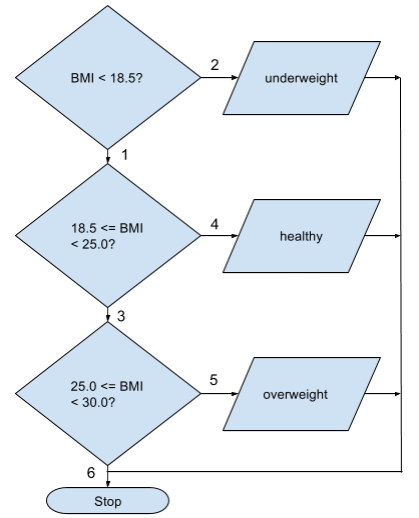
\includegraphics[scale=0.65]{flowchart}
            \caption*{Figure: Decision block of the BMI calculator}
        \end{figure}

        \part Which C++ decision statement would be most appropriate for programming the behavior as shown in the figure?
        \begin{choices}
            \choice \texttt{switch} statement
            \choice nested \texttt{switch} statement (\texttt{switch} within a \texttt{switch})
            \choice \texttt{if} statement
            \choice \texttt{if...else} statement
        \end{choices}

    \end{parts}

\end{questions}
\end{document}